\documentclass{lmcs}
\usepackage{enumerate}
\usepackage{hyperref}
\usepackage{tikz}
\usepackage{listings}
\usepackage{doc}
\usepackage{pgfplots}
\usepackage{pgfplotstable}
\pgfplotsset{compat=newest}

\renewcommand{\arraystretch}{1.3}
\newenvironment{centeredData}{%
    \medskip%
    \begin{center}%
}{%
    \end{center}%
    \medskip%
}

\begin{document}

\title[Citation Indexing]{Citation Indexing:\\ a comparative study of citation access in three services}


\author{Tom\'a\v s Jakl}
\address{School of Computer Science, The University of Birmingham, Edgbaston Birmingham, B15 2TT, United Kingdom}
\email{txj300@cs.bham.ac.uk}
%\thanks{thanks 1, optional.}

\keywords{citation analysis, currency of citation indexing services}
\subjclass{[\textbf{Information storage and retrieval}]: Content Analysis and Indexing---Indexing methods}

\titlecomment{The \LaTeX{} style used is the one required by Logical Methods in Computer Science. The class file can be obtained on~\url{http://www.lmcs-online.org/Information/style.php}.}

\begin{abstract}
  \noindent We try to compare three citation indexing services: Google Scholar, Web of Science and Scopus, based on a quality of data they produce and the data's currency. Also, we take a look at how well the services cover basic literature of Computer Science and how user friendly they are.
\end{abstract}

\maketitle

\section*{Introduction}

As there are more and more people working in science and more and more papers are being published every year, it is an important task to be able to recognise the papers that shine the amongst others and, also, to be able to find relevant information to the problems we are trying to understand.

One of the most important indicators about a paper is its list of citations. In theory, it shows the author's understanding of the topic and its history, and that the author is not doing something that has been already done, but rather that he is able to combine old ideas with new to extend human knowledge. Unfortunately, this is just a theory. Because scientists are often expected to write some amount of papers every year, it is inevitable that an important part of these papers is not of a great quality. And, moreover, in the low-quality papers the authors often cite their old papers or theirs friends paper to gain credit.

To understand how much are citation relevant and to help people to keep track relevant papers, several on-line \emph{citation indexing services} were developed. Just having such tools is not good enough. It is also important to know their strengths and weaknesses.

In this paper, we present important properties of citation indexing services and show how one can measure them. To demonstrate the previous we will analyse the following three services: Google Scholar (GS), Web of Science (WoS) and Scopus (Sc). We would like to answer the questions proposed by Peter Hancox in~\cite{hancox}:

\begin{enumerate}
\item Are there significant differences in the citations retrieved by each of these services?
\item How well does each service provide access to the core forms of literature of Computer Science?
\item What is the currency of each the service?
\item Subjectively, how easy is each of the systems to use?
\end{enumerate}

\bigskip

We are aware of the fact that our resources are limited. The point is just to demonstrate the method and show how it can be used to understand real world data. For a full analysis, one would have to develop more automated systems for both data collecting and data analysis.

\section{Methodology}

For our experiment, we pick a prominent scientist in Computer Science, select five papers he published in 2010 and gather all the papers that cite these five. We do the last step for every service independently. Then, we provide a data analysis of the collected data and compare the three selected citation indexing services.

\section{Papers selecting}

We choose \emph{Gordon Plotkin} as one of the most promiment scientists in the Computer Science. Next, we are suppose to pick five papers he submited in 2010 that are indexed by all three citation serviced we are interested in. However, GS, WoS and Sc agree only on the following four papers published by Gordon Plotkin in 2010\footnotemark:

\footnotetext{For GS, we first find the author and then list all the papers he published. For WoS and Sc, we get better results if we search for papers with author satisfying the query \texttt{"Plotkin, G*"}. This is necessary because Gordon Plotkin's middle name, David, is not always provided.}

\begin{itemize}
\item \emph{Paper 1:} Robin Milner, a Craftsman of Tools for the Mind~\cite{DBLP:conf/lics/Plotkin10},
\item \emph{Paper 2:} A language for biochemical systems: design and formal specification~\cite{DBLP:journals/tcsb/PedersenP10},
\item \emph{Paper 3:} A Model of Cooperative Threads~\cite{DBLP:journals/corr/abs-1009-2405},
\item \emph{Paper 4:} On Protection by Layout Randomization~\cite{DBLP:conf/csfw/AbadiP10}.
\end{itemize}

\noindent
Therefore, we also need to pick one paper from 2009:
\begin{itemize}
\item \emph{Paper 5:} Configuration structures, event structures and Petri nets~\cite{DBLP:journals/corr/abs-0912-4023}.
\end{itemize}

\bigskip

One may object that the reason why we strugled with our choice of the five articles above is because we chose a retird or expired author. But, this is very far from the truth. In theoretical Computer Science it very uncommon to publish more than three papers per year (on avarage) and Gordon Plotkin is definitely  in his best academic years.

\subsection*{Remark}
An another problem we had to tackle was that the citation services often show for a paper a different year of publication. Namely, Paper 3 was published in 2010 but presented in a conferencence in 2009 and Paper 4 was presented at a symphosium in 2010 but published at 2012. GS always considers different copies of a paper as just one, whereas WoS and Sc cosider different versions as different papers. Later, when we analyse citations of these papers, we take into account all citations of all versions of these papers (as GS does).


\section{Citations gathering}

The next step is to gather the most recent ten papers that cite the five papers we selected above. We decided to import the citations into \BibTeX{} databases because, this way, we can use \LaTeX{} itself and a script we wrote to help us analyse the data. The script is provided in Appendix~\ref{app:A}.

Getting a \BibTeX{} database file containing all the papers that cite a particular paper is easy in WoS and Sc. Both tools provide an option to export search queries. GS, on the other hand, does not provide a such comfort. One has to select and export papers one by one.

To remove duplicates we use both \LaTeX{} itself and the script we wrote. For the first, we created a \LaTeX{} script (named \texttt{bibs.tex}) and by changing \texttt{\textbackslash bibliographystyle} options (to \texttt{plain} or \texttt{ieeetr}, for example) we get different orderings of the \BibTeX{} databases and we can search for duplicates. If we believe that our databases are in a good shape (i.e. the exported data are correct), we can do the same automatically with our script.


\section{Analysis}

\subsection{Retrieved data}
To try to answer the first question, we look at how many papers all three databases index and how many do they have in common:

\begin{centeredData}
\begin{tabular}{r|c c c|c c c|c}
         & GS &  WoS & Sc & GS $\cap$ WoS & GS $\cap$ Sc & WoS $\cap$ Sc & WoS $\cap$ GS $\cap$ Sc \\
\hline
Paper 1  &  0 & 0 &  0 & 0 & 0 & 0 & 0 \\
Paper 2  & 10 & 8 & 10 & 4 & 5 & 6 & 4 \\
Paper 3  & 10 & 1 &  4 & 1 & 1 & 0 & 0 \\
Paper 4  & 10 & 1 & 10 & 0 & 5 & 0 & 0 \\
Paper 5  & 10 & 9 & 10 & 3 & 5 & 4 & 2
\end{tabular}
\end{centeredData}

In the table, every row corresponds to a paper, and columns GS, WoS and Sc show how many papers citing the paper corresponding to the row we could find in the particular database. The columns GS $\cap$ WoS, GS $\cap$ Sc, WoS $\cap$ Sc, WoS $\cap$ GS $\cap$ Sc show how many papers are in the corresponding intersection. For better understanding see Figure~\ref{pic:circles}.

Although it looks like that there is very little similarity between the citation search engines, the converse is true. In fact, after inspecting all the data related to Paper 2 more carefuly (not just the last 10 citations but all of them), it is clear that GS indexes all the papers citing Paper 2, and WoS and Sc index just a subset of it.

\begin{figure}[!h]
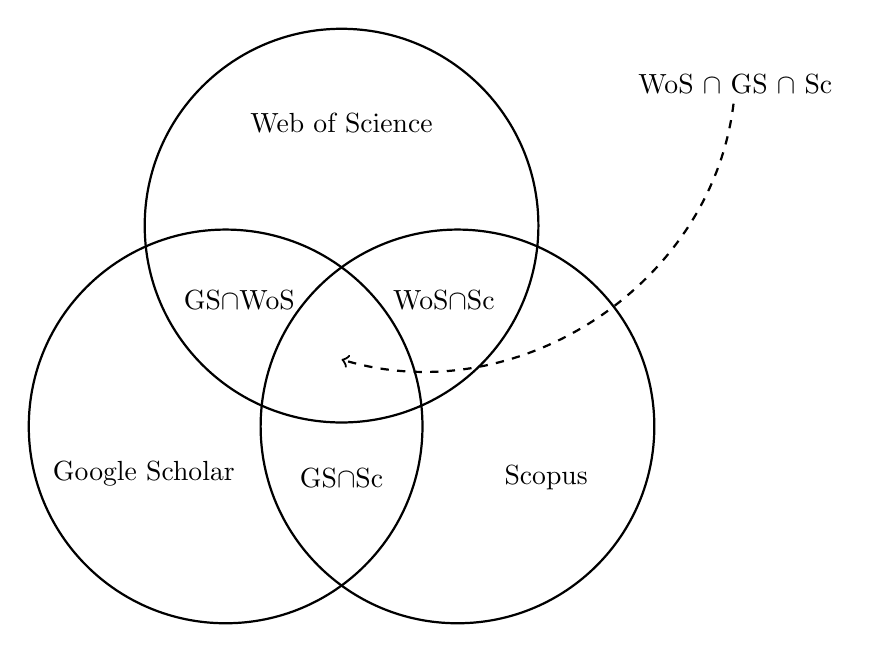
\begin{tikzpicture}[thick]
  \draw  ( 90:1.7) circle (2.5);
  \draw  (210:1.7) circle (2.5);
  \draw  (330:1.7) circle (2.5);

  \node at ( 90:3) { Web of Science };
  \node at (210:2.9) { Google Scholar  };
  \node at (330:3) { Scopus  };

  \node at ( 30:1.5) { WoS$\cap$Sc };
  \node at (150:1.5) { GS$\cap$WoS };
  \node at (270:1.5) { GS$\cap$Sc  };

  \node (all) at (5,3.5) { WoS $\cap$ GS $\cap$ Sc  };
  \path[draw, ->] (all)  edge[bend  left=50, dashed]  node {} (0,0);
\end{tikzpicture}
\caption{Intersections of indexings}
\label{pic:circles}
\end{figure}

\subsection{Forms of literature}

To decide whether an citation search engine covers all the core forms of literature, it is enough to inspect what is the proportion of cited articles, conference papers, technical reports, books and theses. Similarly to previous, we just inspect the data:

\begin{centeredData}
\begin{tabular}{r|c c c c c c|c}
    & Articles & From Conferences & Tech. Reports & Books & Theses & Unknown & Total \\
\hline
GS  & 30 & 5 & 1 & 1 & 2 & 1 & 40 \\
WoS & 9 & 11 & 0 & 0 & 0 & 0 & 20 \\
Sc  & 27 & 8 & 0 & 0 & 0 & 0 & 35
\end{tabular}
\end{centeredData}

It seems that all three services are having problems when indexing technical reports, books and theses. In the first two cases, however, one should not make such a strong statement. First, Gordon Plotkin's interests are very theoretical and we should not expect that many technical reports to even exists. Second, it does not make sense to write a book about a relatively new topic and, again, it may easily happen that no book citing any of the author's papers from 2010 was written in the past 5 years.

\subsection{Currency}

Simply by comparing the average year of publication, one can see that GS should index the most recent papers, and Sc should be the second in currency:

\begin{centeredData}
\begin{tabular}{r|c c c}
         & GS &  WoS & Sc \\
\hline
Paper 2  & 2013.200 & 2011.875 & 2012.400 \\
Paper 3  & 2012.400 & 2012.000 & 2010.250 \\
Paper 4  & 2013.556 & 2011.000 & 2012.636 \\
Paper 5  & 2013.600 & 2012.200 & 2013.000 \\
\hline
Average  & 2013.189 & 2011.769 & 2012.072
\end{tabular}
\end{centeredData}

We get the same conclusion if we take a look at the data more closely and compare the total amount of papers published every single year. See Figure~\ref{pic:years}.

\begin{figure}[!h]
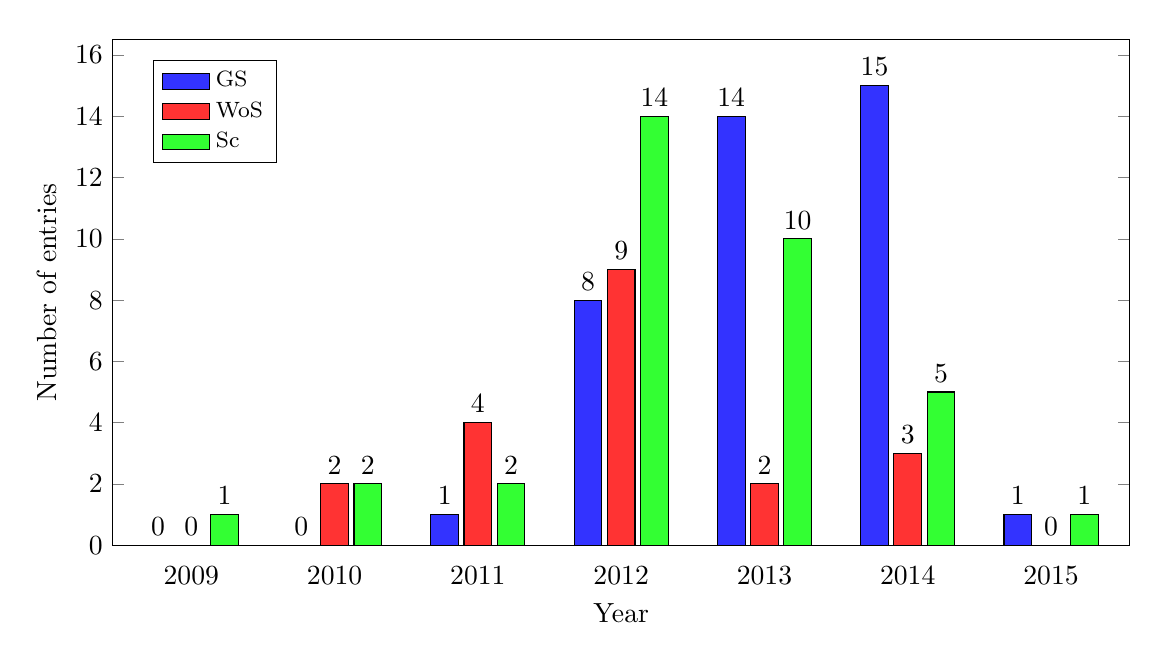
\begin{tikzpicture}
\begin{axis}[
    ybar,
    height=8cm, width=14.5cm,
    ymin=0,ymax=16.5,
    xtick=data,
    enlarge x limits={abs=1cm},
    symbolic x coords={2009, 2010, 2011, 2012, 2013, 2014, 2015},
    bar width = 10pt,
    ylabel= Number of entries,
    xlabel= Year,
    major x tick style = transparent,
    legend style={at={(0.04,0.96)},anchor=north west, font=\footnotesize, legend cell align=left,},
    nodes near coords={
                \pgfmathprintnumber[precision=0]{\pgfplotspointmeta}
                       }
    ]
    \addplot[ybar,fill=blue!80, area legend] coordinates {
        (2009,0)
        (2010,0)
        (2011,1)
        (2012,8)
        (2013,14)
        (2014,15)
        (2015,1)};
    \addplot[ybar,fill=red!80, area legend] coordinates {
        (2009,0)
        (2010,2)
        (2011,4)
        (2012,9)
        (2013,2)
        (2014,3)
        (2015,0)};
    \addplot[ybar,fill=green!80, area legend] coordinates {
        (2009,1)
        (2010,2)
        (2011,2)
        (2012,14)
        (2013,10)
        (2014,5)
        (2015,1)};
    \legend{GS, WoS, Sc}
\end{axis}
\end{tikzpicture}
\caption{Number of citations per year}
\label{pic:years}
\end{figure}


\subsection{Personal opinion}

The last question we would like to address is how user friendly the services are. This is clearly just a subjective comparison and, based on one's preferences, one may easily come up with a different result.

Google Scholar proved to be the best out of the three in data indexing but it is often too greedy. Many times it retrieve preliminary versions of papers from arXiv that were not even published. Also, the fact that it does not allow to export a search makes it useless for a meaningful data analysis. Moreover, query options of GS seems to be very limited. For example, ordering all citations by date shows only those that were published in the last year and there seems to be no way how to extend it to the previous years.

Web of Science, although it provides the most appealing user interface, is very slow and is sometimes hard to make it do what one would want to. For example, one can export searched citations to \BibTeX{} only by going to the page of a particular paper and then listing the papers citing it (skipping the first step and going directly to the papers citing does not allow \BibTeX{} export).

Clear winner in this category is Scopus. The interface is decent looking, easy to work with and the service does what the user asks for.

\section{Conclusion}

There is no clear winner. Google Scholar indexes much more papers than the other two but it does not provide such a good user interface and advanced tools as the others. Also, we did not aim to do a full analysis. For that, it is necessary to gather much more data.

Even with the little explored, it is clear that the current citation indexing services are still at the beginning and better tools need to be developed.

\section*{Acknowledgement}
  The author is grateful to Henning Thielemann for writing the Haskell library \texttt{bibtex} that allowed the analysis to be automatised.

\bibliography{refs}
\bibliographystyle{plain}

\appendix
\section{}
\label{app:A}

Here we provide the Haskell code we used for our analysis. It assumes that all the \BibTeX{} databases are placed in folder \texttt{bibs} and named properly (see the end of the source code for the exact naming convention).

\lstinputlisting[
    language=Haskell,
    basicstyle=\footnotesize,
    breaklines=true,
    showstringspaces=false
    ]{Analyse.hs}

\end{document}

